\begin{longtable} { | c | p{12cm} | c | } 
\hline
	ID 	&	Issues	&		 Es. hours \\\hline
	 67	&	Sequenceviewer: Portrait-mode	&	2 hours \\\hline
\caption{Issue ID 67}
\label{tab:spr4_SVportrait}
\end{longtable}

Portrait-mode is set up in the VerticallyScroll class. The code is very similar to the one in HorizontallyScroll, but there are minor issues remaining before the features developed in other issues are implemented correctly. Portrait-mode has a problem with scaling the pictograms up, making them too large for the dynamic show to work properly. Before Portrait-mode can be considered resolved, this problem has to fixed.

The problem with scaling can be seen in figure \ref{fig:portraitscaling}. The settings are set to display five pictograms in a sequence, but the scaling is clearly not working as intended.

\begin{figure}[H]
	\centering
	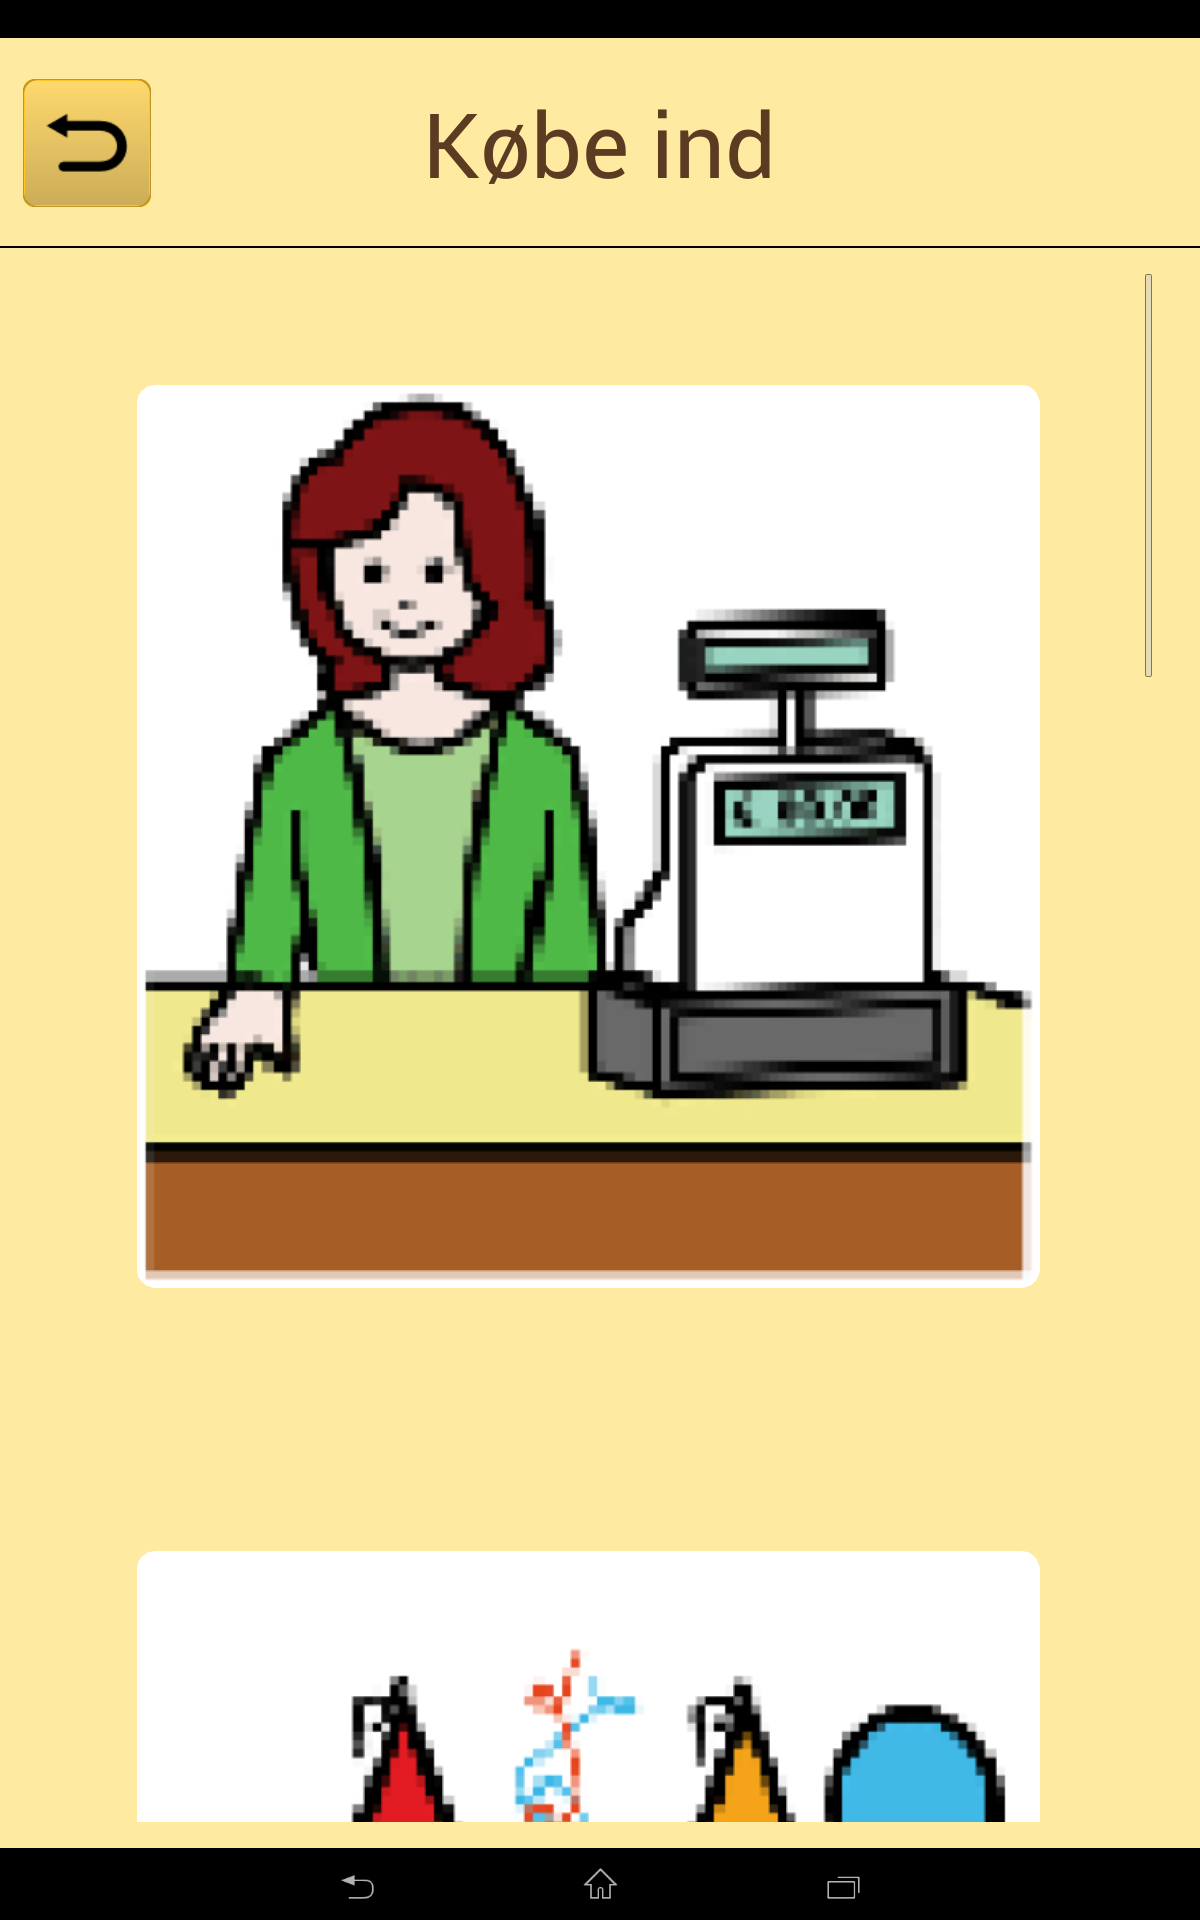
\includegraphics[scale=0.12]{Pics/Sprint4/portraitscaling.png}
	\caption{A sequence displayed in portrait-mode, with the setting set to 5 visible pictograms. The scaling is clearly not working }
	\label{fig:portraitscaling}
\end{figure}